% Chapter 4 -- structure from table of content.md; impersonal academic style; no shallow subsections

\reportchapter{4}{Implementation and Engineering}{NLP extraction, persistence, retrieval and reasoning services, frontend interfaces, deployment, and observability.}

\section{Introduction}

This chapter describes how the design of Chapter~3 was engineered in code, containers, and user-facing interfaces. The presentation covers the NLP and extraction pipeline, polyglot persistence, hybrid retrieval and reasoning services, the React frontend documented through operational screenshots, and the deployment plus observability stack that supports production-like operation. Implementation choices emphasize explicit service boundaries, deterministic identifiers where possible, and traceability from interface actions back to backend evidence. Evaluation against curated benchmarks is deferred to Chapter~5.

\section{NLP Pipeline and Extraction}

Joint entity--relation extraction is orchestrated through DSPy modules calling Mistral in JSON mode. Prompt templates are treated as optimizable modules rather than static strings: the MIPROv2 Bayesian optimizer explores alternative instructions and few-shot examples on controlled batches, then retains the configuration that maximizes a composite extraction score. Reported gains on the project benchmark include approximately \textbf{+2.9\%} on the composite score and roughly \textbf{1.18\,s} lower average inference time per document compared with the initial manual prompt. Offline optimization with DSPy is therefore separated from online serving with the production Mistral client, so prompt iteration does not destabilize the live API.

The extraction contract requires a single pass over each normalized MongoDB document, emitting entities, typed relations, and structured fields aligned with the geopolitical ontology (Chapter~3). Deterministic identifier generation is enforced in prompt logic so that repeated runs map the same canonical actor to the same graph key, preserving topological consistency between MongoDB assertions and Neo4j nodes. Validation rejects malformed JSON, empty extractions, and role titles mistaken for personal names before graph publication. Failed documents remain in MongoDB with explicit error states for administrator inspection rather than silently polluting Neo4j or ZVec indexes.

\section{Persistence Layer Implementation}

\textbf{MongoDB.} Fourteen indexed collections hold documents, chunks, mentions, assertions, structured legislative and financial records, conflict flags, users, chat sessions, messages, and query history. The \texttt{documents} collection carries processing checkpoints (\texttt{graph\_extracted}, \texttt{structured\_extracted}, \texttt{chunks\_created}) that drive idempotent pipeline scripts. Dashboard views and the document library read directly from these collections while keeping application state separate from evidence records.

\textbf{Neo4j.} The property graph enforces ten canonical entity types and thirty-two relationship types. The \texttt{EntityResolutionService} normalizes surface forms, filters verb-like or generic role phrases, maps aliases to canonical types, and assigns stable identifiers before \texttt{MERGE} operations. Traversal queries use parameterized Cypher with depth limits aligned to the design target (up to three hops under nominal load). Graph writes occur only after MongoDB assertions pass schema and quality checks.

\textbf{ZVec.} Embeddings of \texttt{document\_chunks} are stored locally with chunk, document, and entity metadata for hybrid ranking. At query time the backend embeds the user question, retrieves candidates by cosine similarity, and applies lexical reranking before passing chunks to synthesis. Local persistence supports data-sovereignty constraints and removes dependency on an external vector SaaS. Figure~\ref{fig:zvec-performance} summarizes published benchmark characteristics that motivated this choice \cite{zvec-repo,zvec-benchmarks}.

\begin{figure}[H]
    \centering
    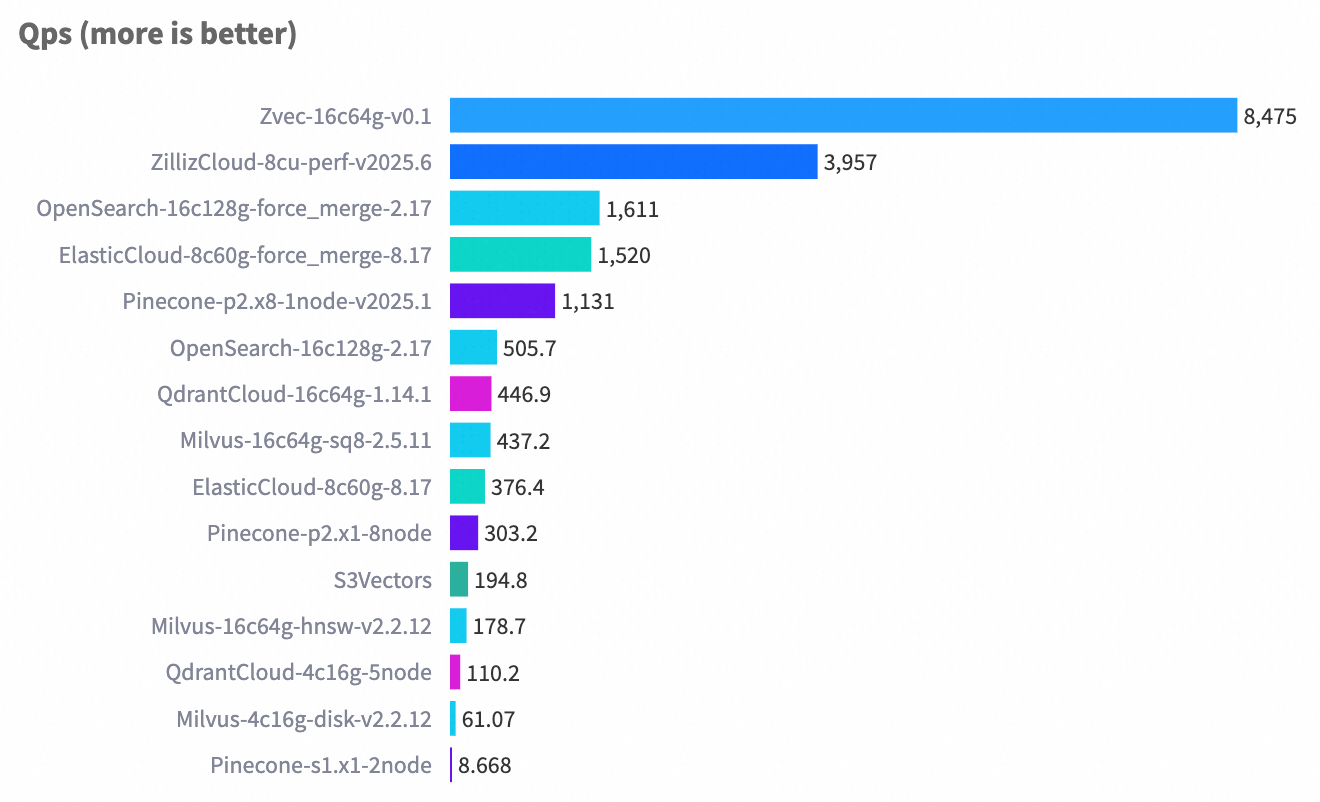
\includegraphics[width=0.92\textwidth,keepaspectratio]{images/zvec Performance at Scale.png}
    \caption{ZVec performance at scale (official benchmark overview).}
    \label{fig:zvec-performance}
\end{figure}

\textbf{Redis.} A cache layer stores reasoning traces, session context, and frequently accessed metadata so repeated analytical sessions remain responsive. Cache entries are keyed by session and query identifiers; invalidation follows session lifecycle events rather than corpus-wide flushes, so ingestion backfills do not unnecessarily evict active conversations.

\section{Retrieval and Reasoning Implementation}

The \texttt{ReasoningEngine} service implements the plan--retrieve--synthesize loop described in Chapter~3. Regardless of mode, the skeleton comprises planning (when enabled), ZVec chunk retrieval, optional Neo4j entity lookup and traversal (depth~2 by default, up to \texttt{MAX\_HOPS = 3} iterations in multi-hop modes), synthesis through Mistral with structured citation fields, and serialization of a reasoning trace for the frontend. Optional web search augments the local corpus when the query signals recency or when the user explicitly enables it.

Figure~\ref{fig:reasoning-modes-implementation} maps the three production modes to retrieval depth. \textbf{RAG mode} skips decomposition and graph expansion: the original question queries ZVec once, chunks are deduplicated, and synthesis proceeds immediately---minimizing latency for factual lookups. \textbf{Chain-of-thought mode} runs the planner, executes sub-questions sequentially, accumulates chunks and graph facts across hops, then synthesizes. \textbf{Reflexive mode} adds an audit step after each hop; insufficient evidence triggers refined retrieval before synthesis. Redis caches traces so the UI can replay steps without recomputation.

\begin{figure}[H]
    \centering
    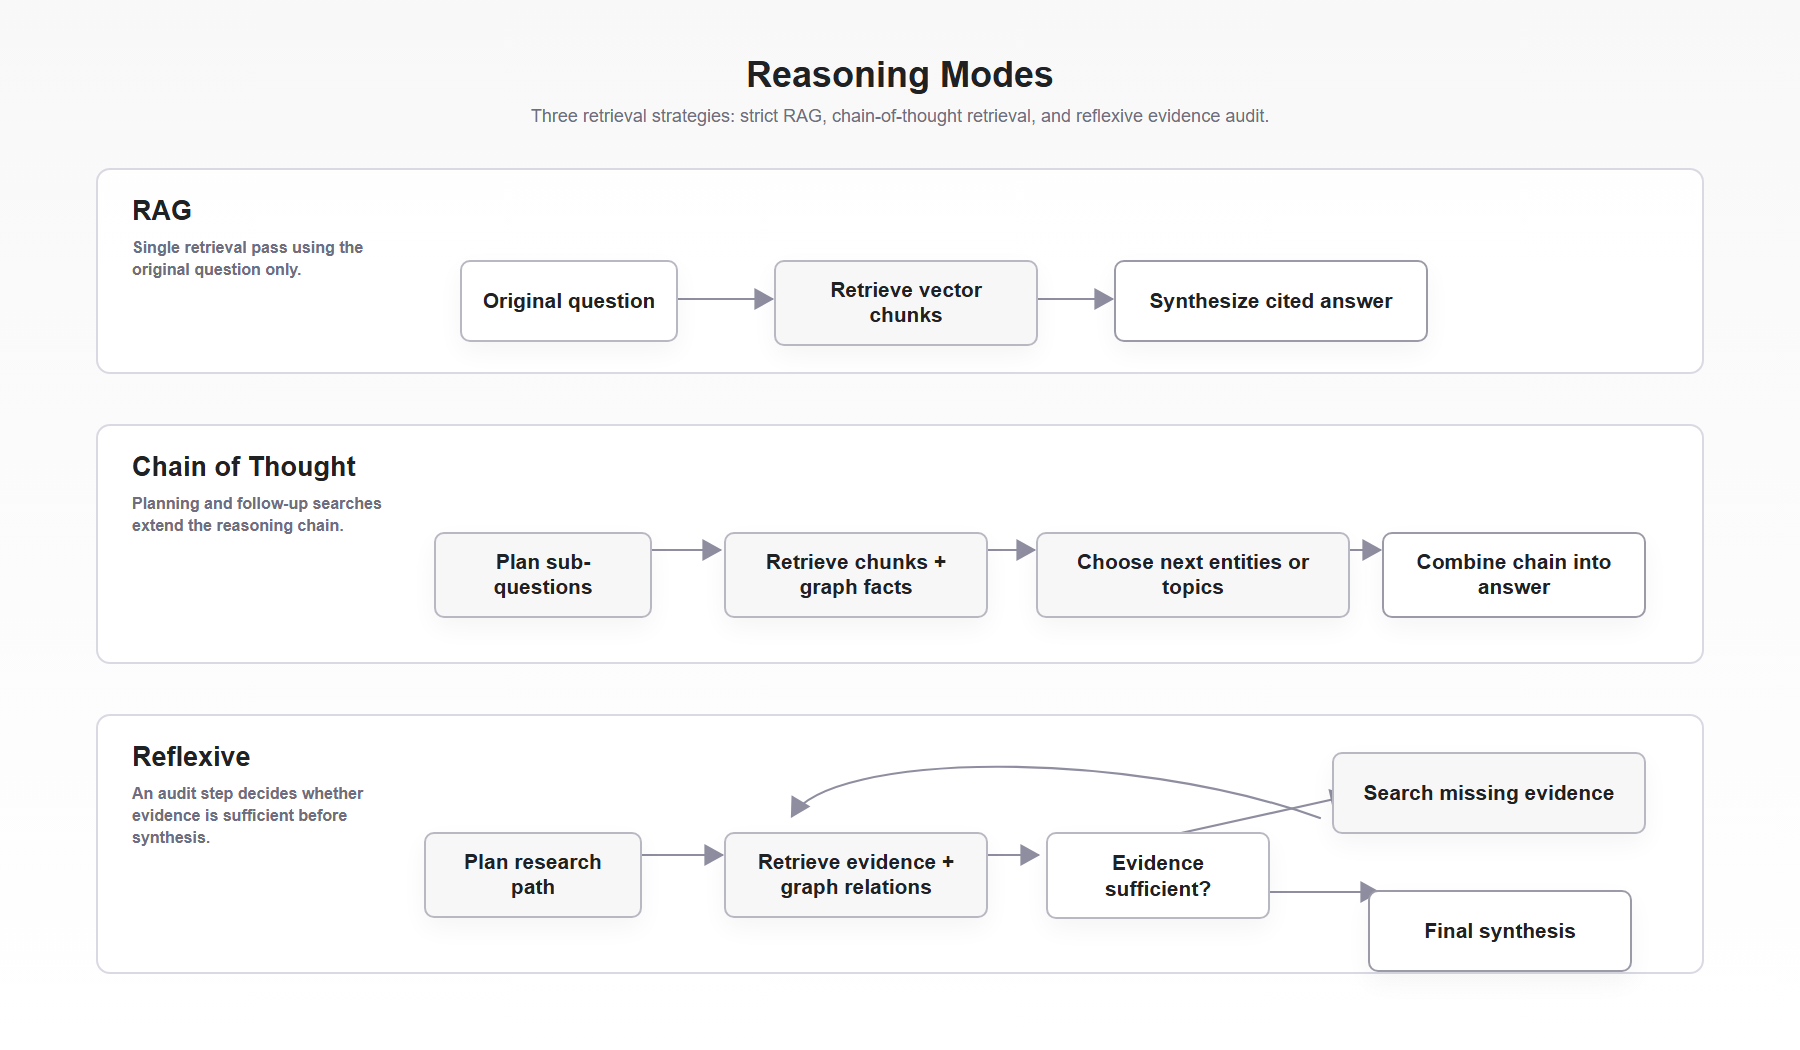
\includegraphics[width=0.96\textwidth,height=0.78\textheight,keepaspectratio]{images/reasoning_modes.png}
    \caption{Three reasoning modes in the query engine: one-hop RAG, chain-of-thought multi-hop, and reflexive control.}
    \label{fig:reasoning-modes-implementation}
\end{figure}

Hybrid ranking combines semantic scores from ZVec, graph distance to seed entities, temporal validity on edges, and deduplication of syndicated passages. Synthesis prompts require explicit source references: chunk identifiers, document titles, and graph fact summaries are passed as structured context. The FastAPI \texttt{/query} route streams thinking steps to the client using server-sent events so the chat interface can render planning, retrieval, audit, and synthesis phases in real time. Chapter~5 evaluates answer quality and grounding across modes on the same deployed endpoint.

\textbf{Optional live web search (DuckDuckGo).} All three reasoning modes can augment the local corpus with external web evidence through \texttt{DuckDuckGoSearchRun} (\texttt{services/websearch.py}). \textbf{DuckDuckGo} is a privacy-oriented search engine: it returns ranked results without user profiling and without a commercial search API key, which aligns with sovereignty constraints and with patterns used by many modern AI agents that combine indexed knowledge with fresh public web pages. The service posts queries to DuckDuckGo's HTML results endpoint (Instant Answer API as fallback), normalizes hits as \texttt{type: web\_search} objects, and passes them to synthesis separately from ZVec chunks so provenance remains explicit. The chat \textbf{Web On / Off} toggle sets \texttt{enable\_web\_search}; recency keywords can auto-enable search; administration exposes \emph{AI Search (DuckDuckGo)} for topic-driven ingestion. Figure~\ref{fig:duckduckgo-rag-websearch} summarizes the implementation flow.

\begin{figure}[H]
    \centering
    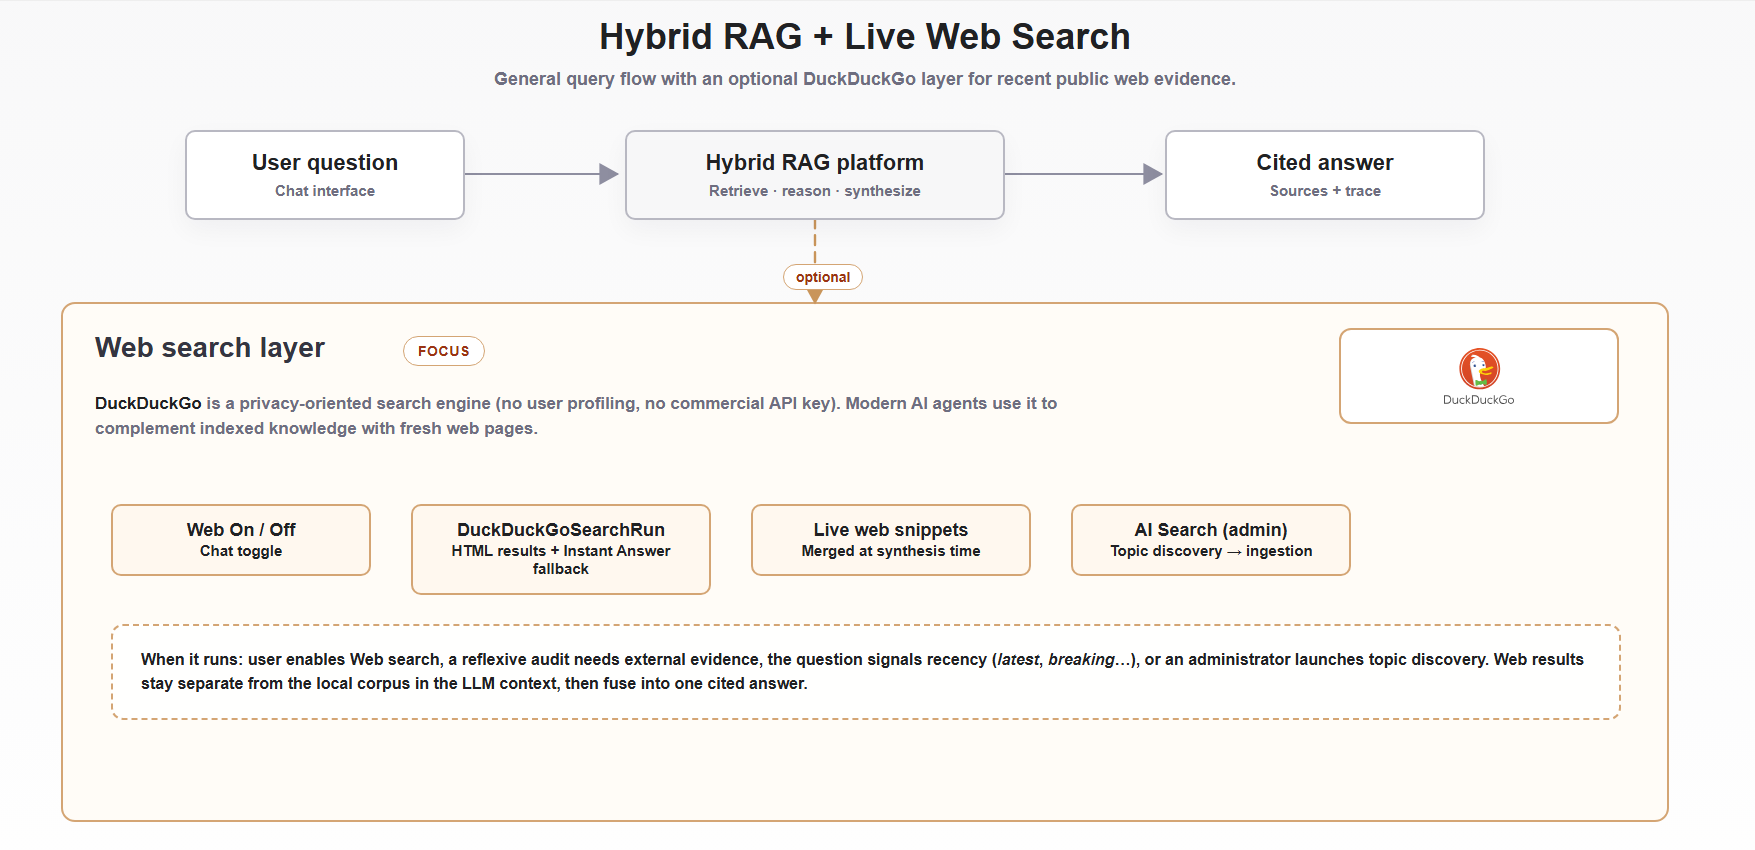
\includegraphics[width=0.96\textwidth,height=0.78\textheight,keepaspectratio]{images/duckduckgo_rag_websearch.png}
    \caption{Hybrid RAG implementation with optional DuckDuckGo web search at query time.}
    \label{fig:duckduckgo-rag-websearch}
\end{figure}

The diagram shows that internal retrieval (ZVec, Neo4j, MongoDB) remains the primary path, while DuckDuckGo supplies supplementary snippets when the user, the reflexive auditor, or an admin discovery job requires information not yet indexed locally. Web evidence does not replace the corpus; it bridges the gap until scheduled ingestion ingests the same sources permanently.

\section{Frontend Implementation}

The client is a React and Vite single-page application with React Router, TanStack Query for server state, and a resizable layout pairing a persistent chat-history sidebar with the active workspace. Routes include the home chat (\texttt{/}), session deep links (\texttt{/chat/:sessionId}), authentication (\texttt{/auth}), administration (\texttt{/admin}), graph explorer (\texttt{/graph}), legislative tracker (\texttt{/legislative/...}), political insights (\texttt{/insights/...}), and document library (\texttt{/documents}). A centralized API client wraps FastAPI endpoints for queries (including SSE streams), graph search, documents, auth, and admin operations, preserving a strict boundary between presentation and backend reasoning services.

\textbf{Analytical workspace: chat and reasoning trace.} The chat interface is the primary entry point for cited questioning. Figure~\ref{fig:ui-chat-interface} shows the layout: session sidebar, message thread, reasoning-mode selector (\texttt{rag}, \texttt{cot}, \texttt{reflexive}), and a \textbf{Web On / Web Off} control linked to DuckDuckGo retrieval in the reasoning implementation above. The mode and web flags are forwarded to the backend as \texttt{reasoning\_mode} and \texttt{enable\_web\_search}.

\begin{figure}[H]
    \centering
    
\includegraphics[width=0.96\textwidth,height=0.72\textheight,keepaspectratio]{chat interface.png}
    \caption{Chat workspace with session history sidebar and reasoning-mode controls.}
    \label{fig:ui-chat-interface}
\end{figure}

Figure~\ref{fig:ui-chat-rag} illustrates a completed answer in RAG mode: the assistant message includes inline citations, source cards, and confidence cues tied to retrieved chunks. Figure~\ref{fig:ui-chat-rag-trace} expands the reasoning trace panel, exposing sequential steps (ZVec retrieval, synthesis) so the user can verify which evidence supported each claim---implementing FR-07 at interface level.

\begin{figure}[H]
    \centering
    
\includegraphics[width=0.96\textwidth,height=0.72\textheight,keepaspectratio]{chat question rag mode.png}
    \caption{Cited answer produced in standard RAG mode with linked source evidence.}
    \label{fig:ui-chat-rag}
\end{figure}

\begin{figure}[H]
    \centering
    
\includegraphics[width=0.96\textwidth,height=0.72\textheight,keepaspectratio]{chat question rag mode reasnoing trace.png}
    \caption{Expandable reasoning trace for a RAG-mode query (retrieval and synthesis steps).}
    \label{fig:ui-chat-rag-trace}
\end{figure}

\textbf{Document library and graph explorer.} The document library (Figure~\ref{fig:ui-documents}) lists ingested sources with filters on metadata, supporting the use case in which analysts verify wording and provenance before trusting synthesized summaries. Selecting a document opens normalized text and extraction status without leaving the analytical shell.

\begin{figure}[H]
    \centering
    
\includegraphics[width=0.96\textwidth,height=0.72\textheight,keepaspectratio]{page documents library.png}
    \caption{Document library for inspecting ingested corpus items and metadata.}
    \label{fig:ui-documents}
\end{figure}

The graph explorer (Figure~\ref{fig:ui-graph}) renders force-directed neighborhoods with \texttt{react-force-graph-2d} and D3.js interactions: pan, zoom, node selection, and typed edge labels. Users pivot from a chat answer to structural exploration by opening the same entities in the graph view, closing the loop between conversational synthesis and relational inspection.

\begin{figure}[H]
    \centering
    
\includegraphics[width=0.96\textwidth,height=0.72\textheight,keepaspectratio]{page graph explorer.png}
    \caption{Graph explorer with interactive entity neighborhood layout.}
    \label{fig:ui-graph}
\end{figure}

\textbf{Legislative and structured political views.} The legislative tracker exposes MongoDB structured records extracted from policy corpora. Figure~\ref{fig:ui-legislative-bills} presents bill listings with status and sponsorship metadata; Figure~\ref{fig:ui-legislative-votes} focuses on roll-call votes; Figure~\ref{fig:ui-legislative-committees} shows committee assignments and related actors. These views complement graph traversal by offering tabular, schema-stable summaries for institutional monitoring.

\begin{figure}[H]
    \centering
    
\includegraphics[width=0.96\textwidth,height=0.72\textheight,keepaspectratio]{page legislative bills.png}
    \caption{Legislative tracker: bills view with structured metadata from extracted records.}
    \label{fig:ui-legislative-bills}
\end{figure}

\begin{figure}[H]
    \centering
    
\includegraphics[width=0.96\textwidth,height=0.72\textheight,keepaspectratio]{page legislative Votes.png}
    \caption{Legislative tracker: votes view linking legislators to roll-call outcomes.}
    \label{fig:ui-legislative-votes}
\end{figure}

\begin{figure}[H]
    \centering
    
\includegraphics[width=0.96\textwidth,height=0.72\textheight,keepaspectratio]{page legislative committes.png}
    \caption{Legislative tracker: committees view for institutional roles and memberships.}
    \label{fig:ui-legislative-committees}
\end{figure}

\textbf{Political insights dashboards.} The \texttt{/insights/...} module groups four analytical tabs on top of MongoDB structured records, Neo4j neighborhoods, and derived analytics services.

The \textbf{finance} tab (Figure~\ref{fig:ui-insights-finance}) queries campaign-contribution and donor records filtered by electoral cycle, country, entity type, and free-text search. It surfaces top donors, aggregated amounts, and finance-related conflict flags when the same actor appears on both sides of a funding relationship---supporting scrutiny of economic influence without leaving the platform.

The \textbf{trends} tab (Figure~\ref{fig:ui-insights-trends}) plots mention frequency and sentiment volatility for entities or topics over selectable windows (e.g.\ seven days) and optional regional filters. Recharts time-series views help analysts distinguish sustained narrative shifts from short-lived spikes in media coverage.

The \textbf{conflicts} tab (Figure~\ref{fig:ui-insights-conflicts}) lists \texttt{conflict\_flags} extracted from documents: opposing stances, shared donors with competing beneficiaries, committee overlaps, and similar patterns where two actors occupy incompatible roles in the evidence. Each row links back to document provenance for manual verification.

The \textbf{compare} tab implements pairwise entity intelligence across eight analytical aspects (or all aspects at once). The user selects two canonical entities via autocomplete (\texttt{/graph/search} suggestions), then chooses an \emph{aspect scope}:
\begin{itemize}[leftmargin=*, itemsep=2pt]
\item \textbf{Political stance} --- party alignment, ideology, support/opposition, coalitions, elections;
\item \textbf{Economic policy} --- budgets, taxation, trade, inflation, subsidies, public spending;
\item \textbf{Influence and network} --- allies, donors, committees, appointments, lobbying ties;
\item \textbf{Governance style} --- reform, transparency, accountability, institutional oversight;
\item \textbf{Legislative record} --- bills, amendments, roll-call votes, committee hearings;
\item \textbf{Foreign policy} --- diplomacy, alliances, sanctions, security treaties;
\item \textbf{Public sentiment} --- polls, approval, protests, media backlash, popularity;
\item \textbf{Risk and conflict exposure} --- scandals, investigations, lawsuits, controversies;
\item \textbf{All aspects} --- runs the full matrix below in one report.
\end{itemize}

Figure~\ref{fig:ui-insights-compare-01} shows the selection panel (two entities + aspect dropdown). The backend (\texttt{POST /political/compare}) resolves both subjects in Neo4j, fetches ZVec/MongoDB evidence filtered by aspect keywords, computes shortest-path graph distance, and builds an \textbf{aspect matrix} (Figure~\ref{fig:ui-insights-compare-02}): for each row, evidence scores for entity~A, entity~B, term overlap, shared neighbors, and graph proximity. Cells summarize how strongly each actor is documented on that dimension.

Figure~\ref{fig:ui-insights-compare-03} presents the narrative layer: \emph{convergences} (shared terms, common neighbors, short graph paths), \emph{divergences} (unique evidence terms and asymmetric neighborhoods), an LLM-generated \emph{conclusion}, and optional \emph{graph path} visualization between the two nodes. The report can be exported as JSON for offline review. This three-step flow---configure, matrix, interpret---mirrors analyst practice: quantify overlap on defined dimensions before drawing qualitative judgments.

\begin{figure}[H]
    \centering
    
\includegraphics[width=0.96\textwidth,height=0.72\textheight,keepaspectratio]{page insights finance.png}
    \caption{Political insights: campaign finance dashboard.}
    \label{fig:ui-insights-finance}
\end{figure}

\begin{figure}[H]
    \centering
    
\includegraphics[width=0.96\textwidth,height=0.72\textheight,keepaspectratio]{page insights trends.png}
    \caption{Political insights: temporal trend tracking for entities or topics.}
    \label{fig:ui-insights-trends}
\end{figure}

\begin{figure}[H]
    \centering
    
\includegraphics[width=0.96\textwidth,height=0.72\textheight,keepaspectratio]{page insights compare 01.png}
    \caption{Entity comparison workflow (step 1): selection of actors or topics to compare.}
    \label{fig:ui-insights-compare-01}
\end{figure}

\begin{figure}[H]
    \centering
    
\includegraphics[width=0.96\textwidth,height=0.72\textheight,keepaspectratio]{page insights compare 02 matrix.png}
    \caption{Entity comparison workflow (step 2): relation matrix between selected entities.}
    \label{fig:ui-insights-compare-02}
\end{figure}

\begin{figure}[H]
    \centering
    
\includegraphics[width=0.96\textwidth,height=0.72\textheight,keepaspectratio]{page insights compare 03 conv div conclusion.png}
    \caption{Entity comparison workflow (step 3): convergence, divergence, and narrative conclusion.}
    \label{fig:ui-insights-compare-03}
\end{figure}

\begin{figure}[H]
    \centering
    
\includegraphics[width=0.96\textwidth,height=0.72\textheight,keepaspectratio]{page insights conflicts.png}
    \caption{Political insights: conflict and opposing-stance visualization.}
    \label{fig:ui-insights-conflicts}
\end{figure}

\textbf{Administration dashboard.} Administrative screens implement supervised ingestion (Chapter~2). Figure~\ref{fig:ui-admin-dashboard} summarizes service health, corpus counts, graph statistics, and recent activity. Figure~\ref{fig:ui-admin-scraped} controls import of scraped JSON batches into MongoDB and backfill into ZVec. Figure~\ref{fig:ui-admin-cron} exposes cron scheduler configuration and agentic trend-collection jobs. Figure~\ref{fig:ui-admin-topic} provides advanced topic search: administrators enter thematic queries that trigger DuckDuckGo-backed discovery (\emph{AI Search}), after which selected URLs follow the standard scrape--normalize--extract pipeline. Together these panels form the operational cockpit of the autonomous crawler rather than a passive monitoring page.

\begin{figure}[H]
    \centering
    
\includegraphics[width=0.96\textwidth,height=0.72\textheight,keepaspectratio]{page admin dashboard.png}
    \caption{Administration dashboard: health metrics, corpus counts, and pipeline overview.}
    \label{fig:ui-admin-dashboard}
\end{figure}

\begin{figure}[H]
    \centering
    
\includegraphics[width=0.96\textwidth,height=0.72\textheight,keepaspectratio]{page admin scaped data ingestion.png}
    \caption{Administration: scraped-data ingestion and vector backfill controls.}
    \label{fig:ui-admin-scraped}
\end{figure}

\begin{figure}[H]
    \centering
    
\includegraphics[width=0.96\textwidth,height=0.72\textheight,keepaspectratio]{page admin cron scheduler control and agnetic trend collector.png}
    \caption{Administration: cron scheduler and agentic trend-collection configuration.}
    \label{fig:ui-admin-cron}
\end{figure}

\begin{figure}[H]
    \centering
    
\includegraphics[width=0.96\textwidth,height=0.72\textheight,keepaspectratio]{page admin advaned topic search.png}
    \caption{Administration: advanced topic search for query-driven source discovery.}
    \label{fig:ui-admin-topic}
\end{figure}

\section{Deployment and Observability}

The stack is orchestrated with Docker Compose: MongoDB, Neo4j, Redis, FastAPI backend, React frontend (nginx), and observability services on a shared bridge network. Health checks on databases gate backend startup so the API does not accept traffic before connectors succeed. Environment variables externalize credentials and model keys, supporting reproducible deployment on sovereign infrastructure without embedding secrets in images.

OpenTelemetry instrumentation exports traces consumed by Jaeger, making multi-hop reasoning visible as a sequence of spans (API entry, retrieval, graph expansion, LLM calls, streaming response). Prometheus scrapes service metrics; Grafana dashboards track query latency, token usage, error rates, and cache behavior. Figure~\ref{fig:observability-stack} summarizes the monitoring topology; Figure~\ref{fig:deployment-topology} shows container relationships in the production compose file.

\begin{figure}[H]
    \centering
    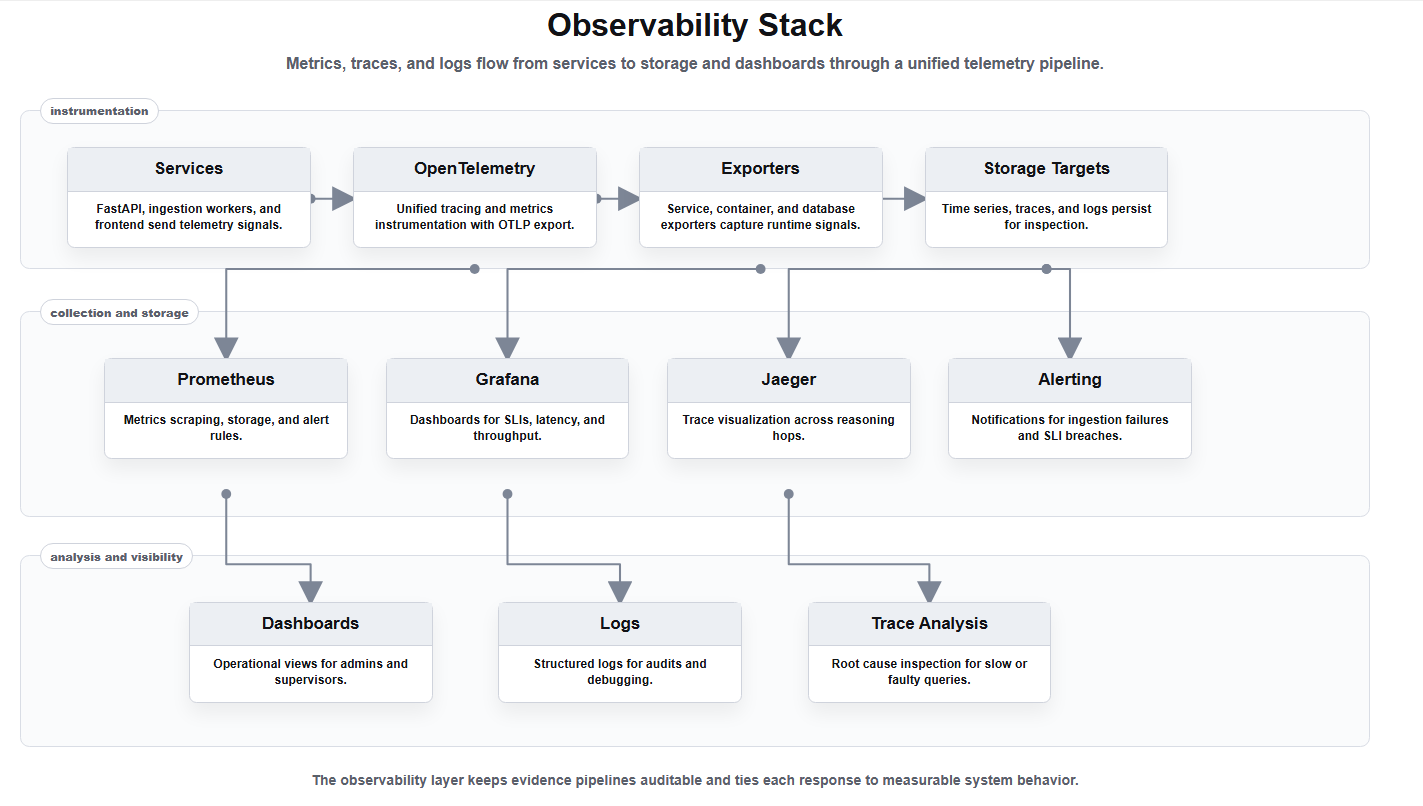
\includegraphics[width=0.96\textwidth,height=0.72\textheight,keepaspectratio]{images/observability_stack.png}
    \caption{Observability stack: metrics, dashboards, and distributed tracing.}
    \label{fig:observability-stack}
\end{figure}

\begin{figure}[H]
    \centering
    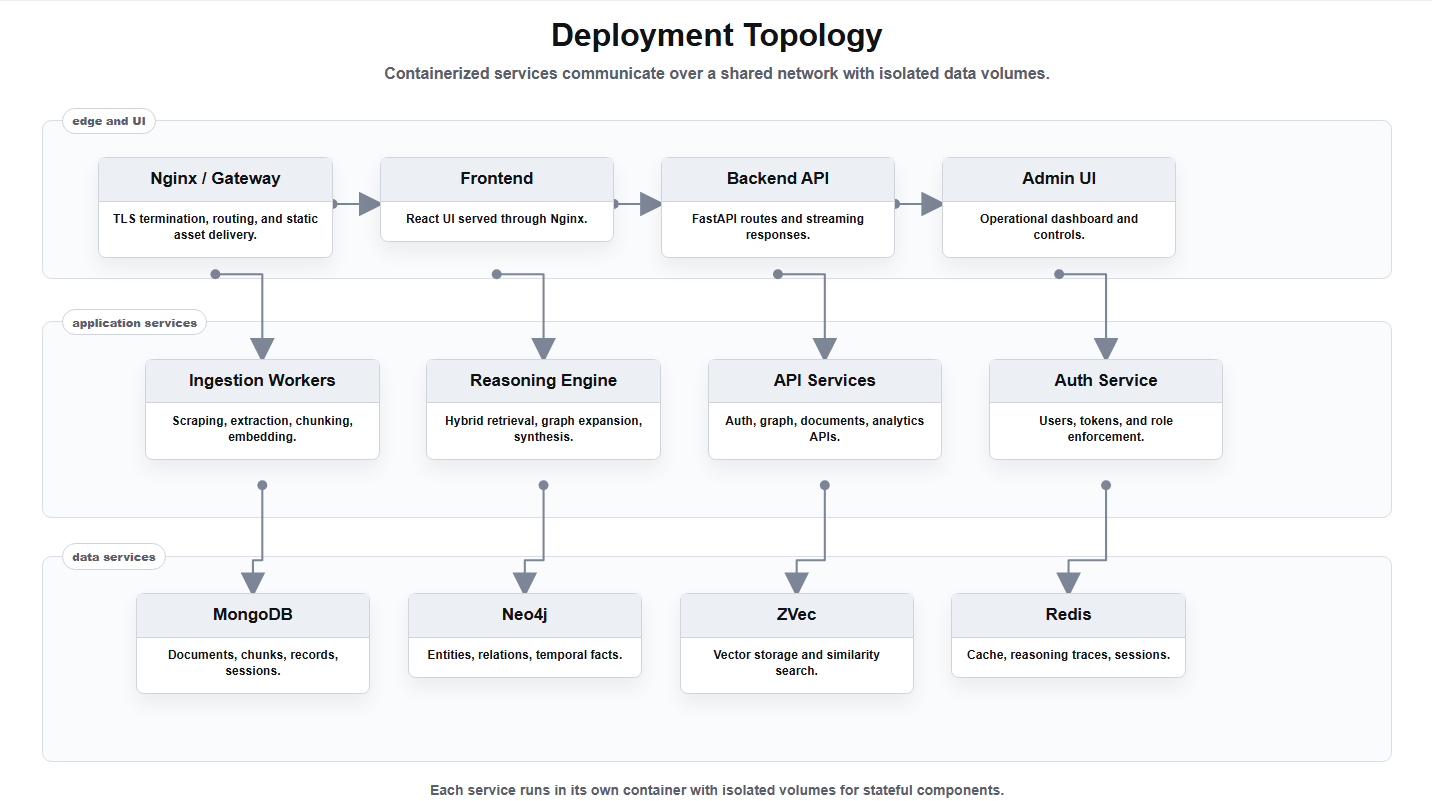
\includegraphics[width=0.96\textwidth,height=0.72\textheight,keepaspectratio]{images/deployment_topology.png}
    \caption{Deployment topology of containerized services and data stores.}
    \label{fig:deployment-topology}
\end{figure}

Resilience measures include API rate limiting with exponential backoff on external LLM calls, inter-document delays during bulk ingestion, graceful degradation when optional services are unavailable, and staged pipeline scripts (graph extract, structured extract, chunk/embed, graph publish) that can be rerun independently. The evaluation harness under \texttt{src/backend/evaluation} calls the same HTTP query endpoint as the frontend, ensuring Chapter~5 measurements reflect deployed behavior rather than isolated unit tests.

\section{Conclusion}

This chapter detailed the engineering realization of the platform: DSPy-optimized extraction, polyglot persistence with local ZVec retrieval, a three-mode reasoning engine with streaming traces, DuckDuckGo-augmented live search, a full React analytical workspace documented through operational screenshots, and a containerized observability stack. The implementation closes the gap between Chapter~3 design artifacts and runnable software. Chapter~5 will report empirical validation against the criteria defined in Chapter~2.
